\chapter{Human-auditable failure analysis and taxonomy development}
\label{ch10-human-auditable-failure-analysis-taxonomy}
In a peer-reviewed study, Zhang et al.~(\href{https://arxiv.org/abs/2505.00212}{2025}) collected expert-annotated failure logs from 127 multi-agent systems, in which several model-driven workers passed work among one another. They then gave the attribution task to the strongest automated methods they could evaluate. The best method identified the responsible agent in 53.5 percent of cases but found the decisive step in only 14.2 percent. Some methods performed below random.

The logs already existed before the attribution problem was posed. Chapter 9 established that recording what happened is necessary, but a complete record does not establish why a run failed. The same trace may support several causal explanations. One worker may introduce a planning error, another may act reasonably on corrupted state, and a third may expose the defect when verification finally runs. Assigning responsibility to the last visible error confuses detection with cause.

Attribution is the scarce capability in this sequence. Logging preserves evidence. Attribution claims that one action materially changed the run's prospects. That claim determines what engineers instrument, which component they repair, whether a benchmark case remains valid, and sometimes who is held accountable. With weak attribution, a complete trace can become a precise record attached to the wrong explanation.

Three practices follow. I derive the initial failure taxonomy from traces produced by the system I operate. I keep a person responsible for consequential causal assignments. I structure the trace so that person can inspect and defend the evidence. Automation can organize and extend the work after those conditions exist. It should not be assumed to create them.

\section{Build the taxonomy from the failures you can inspect}\label{build-the-taxonomy-from-the-failures-you-can-inspect}

The protocol in this section has limited evidentiary support. Its basis is one directional observational study and one practitioner-authored method. Neither is a controlled result showing that the procedure improves an agent system. I still use it because it provides an auditable process for turning local traces into measurement categories. The method comes from Orosz and Husain (\href{https://newsletter.pragmaticengineer.com/p/evals}{2025}), and their recommendation to begin with at least one hundred traces is an unmeasured protocol choice.

I begin with traces from the system and workload I operate. The sample should vary across task type, outcome, model version, repository area, duration, tool use, and any operating condition likely to alter the path through the system. Apparent successes also belong in the sample when verification was skipped or the result depended on an unexplained retry. Excluding them would define failure as only what the current evaluator already detects, preserving the blind spot the review is meant to uncover.

For each trace, I read from the initial request through the terminal state and take open-ended notes. The primary annotation identifies the first upstream failure that materially changed the available path to success. It does not enumerate every later symptom.

A run may begin with an incorrect plan, edit the wrong module, execute a test from the wrong directory, and then misinterpret the failure. Those are four visible defects. If the plan directed all later work toward the wrong module, the planning error is the first upstream failure.

This rule follows the causal structure of an agent run. State moves from one step to the next through messages, files, tool outputs, summaries, and control decisions. An early error changes the evidence and options available downstream. Later actions may therefore be locally reasonable while remaining globally ineffective. Counting every symptom as a separate failure overweights long runs and systems that continue operating after their prospects have already collapsed.

The first-upstream rule also introduces a counterfactual check:

\begin{quote}
If this step had been correct while the preceding record remained unchanged, could the later failure still have occurred through the observed path?
\end{quote}

A clear no makes the step a plausible causal boundary. A yes suggests that the annotation identifies a symptom, or that the trace does not expose enough state to decide. In the latter case, I preserve the uncertainty and leave the causal assignment unresolved.

\begin{figure}[htbp]
\centering
\pandocbounded{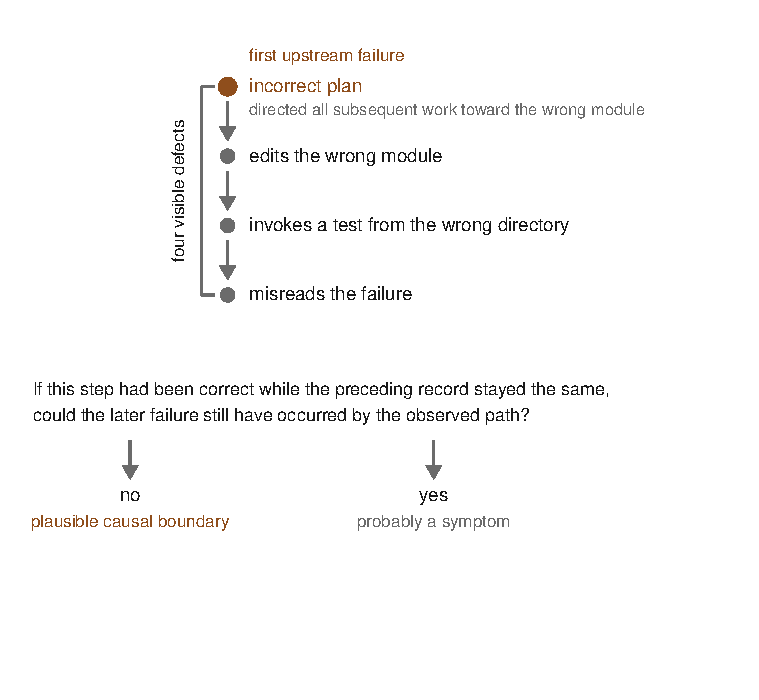
\includegraphics[keepaspectratio,alt={A planning error is the first upstream failure linking four visible defects, while a counterfactual test distinguishes a plausible causal boundary from a symptom.}]{figures/ch10-first-upstream-failure.pdf}}
\caption{A planning error is the first upstream failure linking four visible defects, while a counterfactual test distinguishes a plausible causal boundary from a symptom.}
\end{figure}

The counterfactual holds the preceding record fixed and asks whether the observed path could still have produced the later failure.

After the open review, I cluster the notes into roughly five to ten themes. The categories should describe failures that require different measurement or investigation surfaces. Planning, retrieval, execution, tool use, self-diagnosis, verification, and environment handling may emerge, but I do not impose them before reading the traces. A local pipeline may instead concentrate failures around identity propagation, stale workspace state, permission boundaries, retry ordering, or task ambiguity.

Phase labels are useful because they narrow the evidence required for diagnosis. A planning failure asks whether the system represented the goal, constraints, and dependencies before acting. An execution failure asks whether a valid plan became the intended commands and edits. A self-diagnosis failure asks whether the system interpreted the resulting state correctly. Combining all three under ``reasoning failure'' produces a broad count with little guidance about which part of the trace needs repair.

Generic metric packages often begin with categories that are convenient for the evaluator. They count tool errors because tool errors are easy to parse, or grade final answers because final answers are easy to present to a judge. The resulting dashboard may be internally consistent while missing the upstream decisions that generated those events. A taxonomy derived from traces begins with the failure process and asks only afterward which measurements can represent it.

Published phase-aligned classifications provide useful comparisons. Lu et al.~(\href{https://arxiv.org/abs/2508.13143}{2025}) classified failures by phase across 34 programmable tasks executed by off-the-shelf frameworks operating near 50 percent completion.

Their distribution does not establish base rates for frontier coding agents. It describes the tasks, systems, permissions, and operating point in that study. A production repository with different tools, review gates, task durations, and authority boundaries may concentrate failures elsewhere.

I encountered this mismatch in my own trial-annotation pipeline for experimental agent runs. An early taxonomy omitted failure modes that dominated the project's traces even though public taxonomies covered related categories. The third revision grew from annotation of the local corpus and separated failures along more dimensions. This is narrative illustration only. It does not establish that the resulting taxonomy is complete, and the published export cannot independently reproduce the category counts because its manifest contains no annotations.

The unit of analysis is a complete case. I keep the request, relevant starting state, trace, terminal outcome, verification result, and annotation together. When several retries belong to one attempt, I preserve their order and identities so that a later successful retry does not erase the original failure. When the system forks work, I retain the parent-child relationship. Otherwise an error imported from another branch may appear to originate where it was first observed.

Category boundaries will blur in long, multi-phase work. A retrieval failure can induce a bad plan, while an environment defect can make correct execution resemble faulty reasoning. I allow multiple descriptive tags when they preserve useful context, but retain one first-upstream assignment for frequency analysis. This avoids pretending that causation is always singular while keeping the primary count interpretable.

Reviewer disagreement is evidence about the taxonomy. If two qualified reviewers repeatedly divide the same cases between planning and retrieval, the definitions may depend on state the trace does not expose. If they agree about the events but disagree about the counterfactual, the causal rule needs a sharper boundary. I revise the definitions and preserve the original annotations so the change remains visible.

The initial review of roughly one hundred traces is intentionally laborious. Reading them end to end discovers categories, tests whether the recorded evidence can support those categories, and identifies distinctions that require domain expertise. It cannot estimate a stable low-frequency failure rate with the precision that a larger sample and a \textbf{power analysis} would require. A frequency calculated from one run per task also inherits the run-to-run variation described in Chapter 1, so two nearby categories may reverse order under repetition.

The output of the initial pass is a defensible measurement vocabulary and a labeled seed corpus. Estimating the system's failure distribution requires a separate sampling design.

Once the categories stabilize, scale-out returns to Chapter 5. I validate an LLM-as-judge on a held-out, expert-labeled, stratified sample under the same rubric. I then use it to extend labels only within the operating range supported by its measured errors. The validation belongs to the category definitions in force when it ran. Revising a definition invalidates the agreement estimate for that category.

Human review remains concentrated on new categories, ambiguous cases, consequential failures, and strata in which the automated judge performs poorly. Applying a prebuilt judge before the manual pass would automate someone else's taxonomy rather than discover the failures produced by the local system.

Frequency informs priority without determining it. I count first-upstream assignments by phase and category, examine their uncertainty, and compare their prevalence with the cost of each failure. A frequent, recoverable tool error may deserve less attention than a rare attribution error that invalidates an evaluation. The distribution shows where failures concentrate. Engineering judgment still decides which failures are worth repairing.

Several narrower methods remain in the companion catalog. Constraint-violation logs can localize failure when a task has explicit invariants. Trajectory canonicalization can support structural comparisons across runs. Another entry recommends detecting environment errors before execution because they can consume disproportionate effort. These techniques may sharpen a local taxonomy, but none removes the need to discover which categories the operated system actually produces.

\section{Keep causal assignment under human control}\label{keep-causal-assignment-under-human-control}

Attribution becomes consequential when it changes what happens next. An engineer may rewrite a prompt, repair a tool adapter, remove a benchmark task, retrain a model, or revise an incident report based on the assigned cause. The same label may also affect accountability when different people or services own different parts of the run. In those cases, an automated guess is not a harmless summary.

I separate triage from verdict. Triage ranks cases or candidate steps for investigation. A verdict identifies the responsible action and decisive step, supported by enough evidence that another reviewer can challenge the assignment. Automation can make triage cheaper even when its error rate makes it unsuitable for verdicts.

The opening result shows the current limit. An agent-level accuracy of 53.5 percent leaves nearly half of responsible-agent assignments wrong. A step-level accuracy of 14.2 percent misses the point at which most failures became decisive.

Those figures do not establish a general ceiling for automated attribution. They come from one annotated dataset of multi-agent failures. Single-agent coding traces may be easier, other workloads may be harder, and later methods may improve substantially. The percentages should not be converted into a staffing ratio or a universal automation threshold.

Ma et al.~(\href{https://arxiv.org/abs/2509.08682}{2025}) later reached 36.2 percent step-level accuracy on the same benchmark family, compared with less than 15 percent for prior methods. Counterfactually validated fixes derived from that analysis increased task success by an average of 22.4 percent, although the source does not state whether that gain is absolute or relative. The result suggests that causal structure can narrow the search more effectively than an undifferentiated reading of the transcript. The method still assigned most decisive steps incorrectly.

The fixes were evaluated on the benchmarks that defined the attribution task, and the method required a bespoke causal-discovery algorithm for interaction data whose behavior changes over time. That makes it useful as a candidate generator for a reviewer. It does not justify silently storing its assignment as the postmortem cause.

\Needspace{5\baselineskip}

A human verdict needs a reconstructable chain. I ask:

\begin{itemize}
\tightlist
\item
  Which state changed?
\item
  Which action changed it?
\item
  Which later components consumed that state?
\item
  Which observation eventually exposed the damage?
\end{itemize}

The record must distinguish the actor that introduced the defect from the actor that detected it. It must also distinguish a component that merely propagated invalid state from one that had both the information and the responsibility to reject it.

Consider a run in which a planner selects an obsolete interface, a coding worker implements it faithfully, and a verifier reports an integration failure. The verifier owns the detection. The planner is the first candidate for causal responsibility, provided the current interface was available in the planner's evidence and no later gate explicitly owned the currency check. If the repository index supplied stale documentation, responsibility may move again.

The trace cannot resolve those alternatives unless it records what each step received and what obligation each step owned.

\Needspace{5\baselineskip}

I therefore represent attribution as a structured claim. It records:

\begin{itemize}
\tightlist
\item
  the first upstream action;
\item
  the state transition that action caused;
\item
  the downstream dependency that carried the error;
\item
  the evidence supporting the assignment;
\item
  plausible alternatives considered;
\item
  the reviewer's confidence; and
\item
  the reviewer's identity.
\end{itemize}

This structure does not make the judgment objective. It makes visible where judgment entered. A postmortem that names a ``root cause'' without identifying the state transition behind it is a summary rather than an attribution.

Counterfactual reasoning tests an attribution without proving it. I ask whether replacing the candidate action with a correct one, while holding earlier state fixed, would have prevented the observed failure path. Several steps may satisfy that condition because later checks could also have recovered the run.

Under the taxonomy used here, the decisive step is the earliest point at which the relevant error entered the run or an owned opportunity to stop it was irretrievably missed.

That definition requires an explicit ownership model. A verifier that was never assigned responsibility for checking interface currency should not inherit responsibility merely because it could have caught the error. A release gate whose declared contract includes that check does own a meaningful missed intervention. Postmortems become arbitrary when they infer obligations from hindsight rather than from the contracts active during the run.

Retries complicate attribution because the world may change between attempts. A failed attempt can alter files, caches, rate limits, conversation state, or the evidence presented to the next attempt. A successful retry may depend on those changes, while a later failure may be responding to damage introduced earlier. I preserve attempt identity and state boundaries so reviewers can distinguish a repeated decision from a decision made in a changed environment.

Concurrency creates another ambiguity. Two workers may read the same starting state, make individually valid changes, and conflict only when their outputs merge. Neither branch necessarily contains a unilateral defect. Depending on the violated contract, the failure may belong to the coordination rule, merge order, or missing conflict check. A transcript sorted by completion time can make the worker whose result arrived last appear responsible for a conflict it did not cause.

Before assigning fault to an agent, I rule out the evaluator and execution environment. A broken dependency, stale fixture, permission mismatch, nondeterministic test, or malformed task can make a correct action appear defective. Differential testing runs the same candidate under a controlled change in agent, harness, or environment and asks whether the failure follows the candidate. The companion catalog treats this as a separate diagnostic control because attribution without apparatus checks can turn measurement error into a model failure.

Human control does not require every reviewer to read every trace from the beginning. Automated systems can rank likely decisive steps, group similar incidents, retrieve related cases, prefill observed events, and flag assignments inconsistent with the recorded state transitions. The reviewer remains responsible for accepting, revising, or abstaining. The stored record distinguishes the automated proposal from the signed attribution.

I used the same authority boundary in my internal benchmark-curation process, which determined whether generated software tasks were sound enough to evaluate. Candidate decisions retained an explicit provisional label until a project lead approved them. The pipeline could assemble evidence and run checks, but it could not finalize whether a defect belonged to the task or the evaluated system. This methodology example supplies no accuracy evidence.

The review threshold should follow consequence. A low-stakes transient failure may retain an automated tentative label for aggregate triage. A failure that changes remediation, removes an evaluation item, alters a reported result, or assigns organizational responsibility requires a named human decision.

When the evidence cannot distinguish among plausible causes, the correct verdict is unresolved. The record should state which missing observation would have separated them.

Aggregating several automated readers does not by itself make attribution reliable. The companion catalog describes independent attribution judges as an aside, but agreement among several weak or dependent readers does not establish causation. It also treats consistency across repeated runs as a risk signal. Both may help decide where a person looks first. Neither should determine what that person must conclude.

Repeated local categories can eventually expose a structural defect. When the same failure class survives prompt patches and model upgrades, the remedy is likely architectural, and Chapter 17 develops that redesign question. This chapter stops at diagnosis because recurrence alone does not establish the correct intervention.

\section{Design the record for a skeptical reader}\label{design-the-record-for-a-skeptical-reader}

Deshpande et al.~(\href{https://arxiv.org/abs/2505.08638}{2025}) reported that the strongest evaluated long-context model correctly localized issues in 11 percent of 148 expert-annotated traces. The traces were benchmark-derived but ecologically valid and more complex than short synthetic sequences designed to isolate one error. Reasoning, tool calls, outputs, retries, and state changes appeared in the same record. A large context window could contain the transcript, but containment did not make the decisive event legible.

\begin{figure}[htbp]
\centering
\pandocbounded{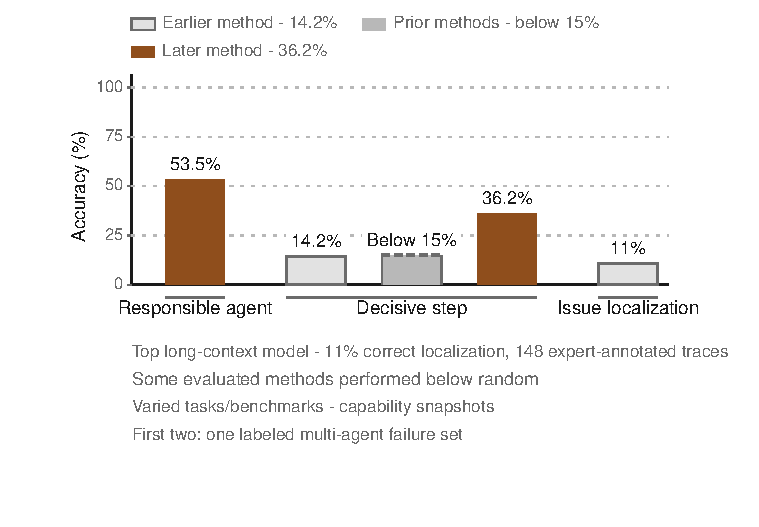
\includegraphics[keepaspectratio,alt={Responsible-agent attribution is 53.5\%; decisive-step attribution is 14.2\% earlier, below 15\% for prior methods, and 36.2\% later; the top long-context model localizes 11\% of 148 traces, and some methods underperform random.}]{figures/ch10-attribution-accuracy.pdf}}
\caption{Responsible-agent attribution is 53.5\%; decisive-step attribution is 14.2\% earlier, below 15\% for prior methods, and 36.2\% later; the top long-context model localizes 11\% of 148 traces, and some methods underperform random.}
\end{figure}

These results span different tasks and benchmarks. The first two use one annotated dataset of multi-agent failures. They are capability snapshots, not a general automation ceiling.

The model scores will change as trace readers improve, and the benchmark cannot establish performance for every production workload. The more durable implication comes from the structure of the task. A record built for human audit should expose the units a causal investigation requires. Raw chronological text forces every reader, human or model, to reconstruct those units before diagnosis begins.

Chapter 9's typed event stream supported replay and recovery. Human audit adds a different requirement. A reviewer must be able to follow step boundaries, decisions, inputs, state transitions, retries, and outcomes without inferring their identities from prose. The same event stream can support both purposes when its schema records semantic boundaries. Timestamps on messages alone do not preserve them.

\Needspace{5\baselineskip}

At minimum, I retain:

\begin{itemize}
\tightlist
\item
  a run identifier;
\item
  the task identity;
\item
  model and configuration versions;
\item
  an initial-state reference; and
\item
  ordered step identifiers.
\end{itemize}

\Needspace{5\baselineskip}

Each step records:

\begin{itemize}
\tightlist
\item
  the actor;
\item
  input references;
\item
  the decision or intended action;
\item
  the tool request;
\item
  the tool response;
\item
  the resulting state reference;
\item
  the verification outcome; and
\item
  the terminal status.
\end{itemize}

Retries identify the attempt they repeat and the reason the controller authorized another attempt. Forks and joins preserve parentage and ordering constraints.

A tool response, file digest, exit status, or test result is an observation. A model statement that the response means a dependency is missing is an interpretation. Storing both under a generic message field encourages later readers to treat the interpretation as though it came from the environment. Typed events allow the reviewer to compare the claim with the observation on which it rests.

Decision records need enough input to reevaluate the choice. A label such as ``selected tool A'' records the outcome but omits the alternatives, constraints, and evidence available at the time. I preserve the relevant input references, selected action, rejected alternatives when the system represented them, and the rule or model version that made the selection.

Replay means re-running or reevaluating a decision against the same recorded inputs. Asking a model to invent a retrospective rationale is a different operation.

Some inputs cannot be stored in full. Repository snapshots, retrieved documents, and tool outputs may be large, sensitive, or mutable. The trace can instead retain content-addressed references, access-controlled snapshots, or a precise query together with the identities of the returned items. A pointer to ``current repository state'' is insufficient because the state will change before review. The preservation policy must balance reproducibility with confidentiality, storage cost, and retention obligations.

Step boundaries should correspond to ownership and state transitions visible to the control plane. One step containing plan generation, three tool calls, an edit, and verification is too coarse for attribution. Recording every token or streaming fragment produces the opposite failure: thousands of events without a meaningful decision boundary.

I use the smallest unit in which one actor receives a defined input and produces an action or state transition consumed by another component.

\Needspace{5\baselineskip}

Tool-call records need more than a name and final output. They should include:

\begin{itemize}
\tightlist
\item
  normalized arguments;
\item
  execution-environment identity;
\item
  start and completion status;
\item
  timeout or cancellation state;
\item
  a summary of side effects; and
\item
  links to resulting artifacts.
\end{itemize}

A command can return a nonzero exit status after partially changing the environment. Recording only the failure status hides files, processes, or external effects inherited by the retry.

Ordering also needs explicit semantics when work overlaps. Wall-clock timestamps help diagnose latency, but clock order does not establish causality across concurrent workers. Parent identifiers, message sequence numbers, versioned state references, and join events show which observations were available to each decision. When two steps race to modify the same artifact, the trace should identify the accepted version and the rule that rejected or merged the other.

Identity must remain stable across resumed work. A display name such as \texttt{coder} may refer to different model versions, sessions, or permission sets. The audit record links the logical role to a particular execution instance, configuration, authority set, and parent run. This lets a reviewer determine whether an outcome changed because of a new decision, a new actor, or state inherited across a restart.

The review interface should support competing explanations. A reviewer should be able to move from an annotated failure to the suspected upstream event, inspect its input state, follow affected descendants, and compare a neighboring successful run. Filtering by actor or event type is useful, but the default view should preserve causal context around each selection. A viewer that hides retries or collapses repeated tool output may improve readability by removing the evidence under dispute.

CodeProbe (\href{https://github.com/sjarmak/codeprobe}{public repository}) publishes complete transcripts and preserves quarantined runs separately. Its successor adds a side-by-side trace browser for audited comparisons. These choices illustrate preservation and review practices. They do not establish that the schema is optimal, and publication alone does not prevent incorrect conclusions.

Quarantined runs are worth preserving because evaluation pipelines often remove timeouts, rate limits, infrastructure failures, and malformed outputs before analysis. Some exclusions are methodologically justified, but deletion prevents a later reviewer from distinguishing an agent failure from an apparatus failure. I retain the raw run, exclusion reason, decision owner, and any replacement attempt. Aggregate reporting can then follow the declared policy without erasing the cases that test it.

Structured traces also improve privacy controls because sensitive fields become identifiable. Credentials, personal data, proprietary source, and private model reasoning may require redaction or restricted access. Blanket retention creates a security liability, while blanket deletion destroys auditability. Field-level policies can restrict access, encrypt retained data, and irreversibly redact secrets. The record should distinguish evidence withheld by policy from evidence the system never captured.

The trace schema must record its own version. Adding a field changes what can be inferred from later runs. Renaming an event can break comparisons with the existing failure corpus. A missing field may mean that the event did not occur, that the recorder omitted it, or that an older schema represented it differently. The decoder and migration logic should distinguish those states explicitly.

Instrumentation can also change the system being observed. Synchronous logging adds latency. Large payloads can alter token budgets, memory use, or rate-limit behavior. Asynchronous emission can reorder records or lose the final buffer during a crash. I measure the overhead, assign a durability requirement to each event class, and record missing events as trace failures. A gap must remain visible in the reconstructed record.

Changing instrumentation between experimental arms also changes the apparatus, which Chapter 1 requires to remain fixed in a paired comparison.

The practitioner evidence for this practice is anecdotal. One organization reported that reviews had consisted of competing opinions until the system began recording decisions, inputs, retries, and outcomes. The resulting structure made failures repeatable and disputes more factual. A second practitioner independently described event-sourced, replayable traces. Both are self-reported accounts. They demonstrate plausible operational use but no controlled improvement or universal schema.

Logging does not repair an agent. It makes causal explanations testable against preserved events and makes repeated failure paths comparable. Repair still requires a separate intervention and an evaluation showing that the intervention changed the intended outcome. This distinction prevents observability work from receiving credit for reliability gains it has only made possible to measure.

The schema should evolve from failed investigations. Common gaps concern the state a worker observed, side effects inherited by a retry, the branch selected at a join, or the evidence behind a decision. I record the unanswered question as an instrumentation defect. The next schema version adds the smallest event or relation that would have answered it. This ties auditability to real investigations and limits speculative completeness.

Trajectory shape can provide an early signal while a run remains active. The companion catalog describes monitoring duration, variance, tool-call count, and other structural changes because failed trajectories may run longer or become more variable. Such a signal can preserve a suspicious run or request earlier review. It cannot identify the cause without the structured events that explain what occurred inside that shape.

\section{Turn failed runs into an operating record}\label{turn-failed-runs-into-an-operating-record}

I begin with the twenty most recent failed runs and read each one from the initial request through the terminal state. My notes remain open-ended, and each case receives one primary assignment: the first upstream failure that materially changed its path to success. I also include apparent successes whose verification was skipped, because an unverified outcome cannot provide clean evidence of success.

This first batch tests the trace as much as the system. It shows whether the record can answer ordinary causal questions before a larger annotation effort depends on it.

I then expand the corpus toward one hundred traces selected across task types, outcomes, model versions, repositories, durations, tools, and operating conditions. I cluster the notes into roughly five to ten failure classes. Their observed frequency helps determine which classes to measure first, while consequence and repair cost determine the final priority.

A named human signs any attribution that changes remediation, accountability, task validity, or the interpretation of an evaluation result. Automated readers may rank the review queue, retrieve related cases, and propose candidate decisive steps. They do not finalize the causal assignment.

The first question the trace cannot answer becomes an instrumentation requirement. I add the missing state reference, event boundary, identity, ordering relation, or outcome field, then preserve the new schema version with later runs. Failed analysis therefore becomes evidence about the observability system itself.

A completed review should state both what the evidence supports and what remains unresolved.

The failure corpus remains an operating asset after Part III. Chapter 14 uses it to tune compaction policy, because compression should preserve the evidence that prior investigations found decisive.

Part IV turns to the evidence available when the model acts: retrieval, context budgets, and memory. Chapter 11 begins by measuring repository retrieval, the first step in deciding which parts of a codebase enter that evidence.

\section*{Sources and evidence}

The evidence grouping on each entry below comes from its catalog record. Author-system cases in this chapter are narrative illustration and are not part of the evidence base.

\textbf{Derive the failure taxonomy from your own traces}

\begin{itemize}
\tightlist
\item
  Directional evidence: Lu, R., Li, Y., Huo, Y. (2025), ``Exploring Autonomous Agents: A Closer Look at Why They Fail When Completing Tasks,'' arXiv:2508.13143. (Phase-aligned classification; \textasciitilde50\% completion base rate on 34 programmable tasks with off-the-shelf frameworks; not an estimate for production repositories.)
\item
  Directional evidence: ``A pragmatic guide to LLM evals for devs'', Gergely Orosz with Hamel Husain, Pragmatic Engineer newsletter, 2025-12-02, \url{https://newsletter.pragmaticengineer.com/p/evals}. (Open coding on 100+ traces, first upstream failure, axial coding into 5-10 themes, prioritize by frequency.)
\end{itemize}

\textbf{Keep humans in failure attribution}

\begin{itemize}
\tightlist
\item
  Strong evidence: Zhang, S., et al.~(2025), ``Which Agent Causes Task Failures and When? On Automated Failure Attribution of LLM Multi-Agent Systems,'' ICML 2025, arXiv:2505.00212. (Who\&When: expert-annotated failure logs from 127 multi-agent systems; 53.5\% agent-level and 14.2\% step-level for the best automated method; some methods below random.)
\item
  Directional evidence: Ma, G., et al.~(2025), ``Automatic Failure Attribution and Critical Step Prediction Method for Multi-Agent Systems Based on Causal Inference,'' arXiv:2509.08682 (CDC-MAS). (36.2\% step-level against under 15\% for prior methods; counterfactually validated fixes worth an average 22.4\% task success.)
\end{itemize}

\textbf{Design traces for human audit}

\begin{itemize}
\tightlist
\item
  Strong evidence: Deshpande, D., et al.~(2025), ``TRAIL: Trace Reasoning and Agentic Issue Localization,'' Patronus AI, arXiv:2505.08638. (Best evaluated model localized issues in 11\% of 148 expert-annotated traces; a 2025 capability snapshot.)
\item
  Corroborating case: ``What actually broke when we put AI agents into real production workflows'', /u/saurabhjain1592, r/LLMDevs, 2026-01-08.
\end{itemize}

\textbf{Author-system illustration cited inline}

\begin{itemize}
\tightlist
\item
  Not an evidence item: CodeProbe, the author's task-mining evaluation tool, \href{https://github.com/sjarmak/codeprobe}{public repository}. Named inline for the published transcripts and quarantined runs described above, which are narrative illustration.
\end{itemize}
